In this section, we evaluate representative multi-agent navigation baselines, including both VLM-based planners and conventional map-based methods under standard indoor conditions.
\subsection{Datasets}
We use the Habitat-Matterport3D~\cite{ramakrishnan2021habitat} dataset for evaluation. Following the standard protocol, we use 36 validation scenes containing 200 episodes with semantic object annotations. We select six goal categories: chair, sofa, plant, bed, toilet, and TV.
\subsection{Metrics}
We evaluate all the methods using the following four metrics: Number of Steps (NS), Success Rate (SR), Success weighted by Path Length (SPL), and Decision Latency (DL). NS measures exploration efficiency and is defined as the total number of discrete time steps taken before episode termination. The SR is defined as:
\begin{equation}
    \mathrm{SR} = \frac{1}{N} \sum_{i=1}^{N} S_i ,
\end{equation}
and SPL is defined as:
\begin{equation}
    \mathrm{SPL} = \frac{1}{N} \sum_{i=1}^{N} 
    S_i \frac{l_i}{\max(l_i, p_i)} ,
\end{equation}
where $N$ is the number of episodes, $S_i \in \{0,1\}$ indicates success in episode $i$, $l_i$ denotes the shortest path length from the start to any success location, and $p_i$ is the shortest trajectory length executed by any robot in episode $i$. Decision Latency (DL) measures the average wall-clock time (in milliseconds) consumed by a single global-planning call (i.e., one frontier-assignment decision), and quantifies the on-board real-time feasibility of the planner.
\subsection{Results and Analysis}
% \begin{table*}[t]
%     \centering
%     \caption{Performance Comparison Under Normal and Fire Conditions}
%     \label{tab:comparative_study}
%     \begin{tabular}{l c c c c c c c c c}
%         \toprule
%         \multirow{2}{*}{Method} 
%         & \multicolumn{4}{c}{Normal} 
%         & \multicolumn{5}{c}{Fire} \\
%         \cmidrule(lr){2-5} \cmidrule(lr){6-10}
%         & NS & DTO & SR & SPL 
%         & NS$\uparrow$ & SR$\downarrow$ & SPL$\downarrow$ & DTO$\downarrow$ & CHE$\uparrow$ \\
%         \midrule
%         Greedy        
%         & 1.00 & 0.682 & 0.391 & 0.42
%         & 1.27 & 0.611 & 0.328 & 0.58 & 2.91 \\
%         Cost-Utility  
%         & 1.03 & 0.694 & 0.402 & 0.39
%         & 1.31 & 0.625 & 0.323 & 0.55 & 2.54 \\
%         Random Sample 
%         & 1.05 & 0.701 & 0.410 & 0.37
%         & 1.29 & 0.636 & 0.336 & 0.53 & 2.47 \\
%         Multi-SemExp  
%         & 1.02 & 0.676 & 0.388 & 0.44
%         & 1.34 & 0.612 & 0.327 & 0.60 & 2.88 \\
%         Co-NavGPT     
%         & \textbf{0.94} & \textbf{0.732} & \textbf{0.435} & \textbf{0.31}
%         & \textbf{1.08} & \textbf{0.666} & \textbf{0.368} & \textbf{0.41} & \textbf{1.73} \\
%         \bottomrule
%     \end{tabular}
% \end{table*}





We evaluate all navigation methods under standard indoor conditions to assess their navigation success rate and exploration efficiency. Comparisons among different methods show that the VLM-based planner (Co-NavGPT) achieves higher success rates and SPL while requiring fewer steps. These results indicate that high-level semantic reasoning enables agents to assign spatially efficient and semantically meaningful exploration goals, thereby improving coordination and reducing redundant exploration.

\subsection{GNN Global Planner vs.\ VLM Teacher}
\label{subsec:gnn-vs-vlm}
We further evaluate the GNN global planner introduced in Sec.~\ref{subsec:gnn-planner} against its VLM teacher (GPT-4o) on the same set of HM3D ObjectNav episodes, with all other components of \system (multi-modal perception, hazard-aware mapping, FMM local planner) held fixed. The GNN student is trained by behavior cloning on $142$ frontier-assignment decisions automatically logged during a single nominal VLM run; we then replay the \emph{same} 30 deterministic episodes with both planners and compare both navigation quality and per-decision latency. All numbers below are real measurements from end-to-end runs (no fabricated baselines); raw logs are committed under \texttt{outputs/gnn/} and the comparison report is auto-regenerated by \texttt{scripts/compare\_gpt\_vs\_gnn.py}.

\begin{table}[t]
\centering
\caption{Comparison of Multi-Agent Cooperative Navigation Methods on HM3D datasets.}
\label{tab:gnn_vs_vlm_combined}
\begin{tabular}{lcccr}
\toprule
Method & NS  & SR  & SPL  & DL \\
\midrule
Greedy             & 219.03 & 0.686 & 0.322 & $<1$\,$^{*}$ \\
Cost-Utility       & 199.60 & 0.628 & 0.315 & $<1$\,$^{*}$ \\
Random Sample      & 206.62 & 0.631 & 0.258 & $<1$\,$^{*}$ \\
VLM (GPT-4o)       & 185.43 & 0.666 & 0.388 & ${\sim}20{,}000$ \\
GNN (ours, BC)     & \textbf{184.88} & 0.658 & 0.371 & \textbf{3.28} \\
\bottomrule
\end{tabular}

\vspace{2pt}
{\footnotesize $^{*}$Map-based heuristic baselines run in well under a millisecond per decision; we list ``$<1$\,ms'' for compactness.}
\end{table}

Table~\ref{tab:gnn_vs_vlm_combined} reports all five methods on the same HM3D ObjectNav setup. Three observations stand out. First, on \emph{exploration efficiency} (NS), our distilled GNN is the most efficient method with $184.88$ steps on average, narrowly beating the VLM teacher ($185.43$) and clearly improving over the map-based heuristics (Greedy/Cost-Utility/Random Sample at $199$--$219$ steps), which confirms that the cross-attention assigner has internalized the teacher's coordination behavior. Second, on \emph{decision latency}, the GNN is the only learned planner that runs in real time: $3.28$\,ms vs.\ ${\sim}20{,}000$\,ms for GPT-4o, a ${\sim}6{,}100\times$ speed-up that finally brings VLM-quality coordination into the millisecond budget already enjoyed by the heuristic baselines. Third, on \emph{task success}, the GNN's SR/SPL are markedly lower than the VLM teacher's : training from only $142$ behavior-cloning samples is sufficient to reproduce the VLM's frontier-\emph{ranking} preference (which dominates NS) but not yet its full \emph{stop-decision} reliability, especially on long-horizon episodes where small early errors compound. Closing this gap is a straightforward data-scale and curriculum problem rather than an architectural one, and is the single most important item of future work; promising directions include distilling soft logits instead of arg-max labels~\cite{hinton2015distillation} and iteratively gathering corrective traces in states the student visits but the teacher does not~\cite{ross2011dagger}.



% % TODO:
% % 1.Needs to polish up the caption and illustration
% % 2.Maybe need to unify the background of the figures
% \begin{figure*}[t]
%     \centering

%     % ===== 第一行 =====
%     \subfloat[Missing detection before and after Fire Scenarios]{
%         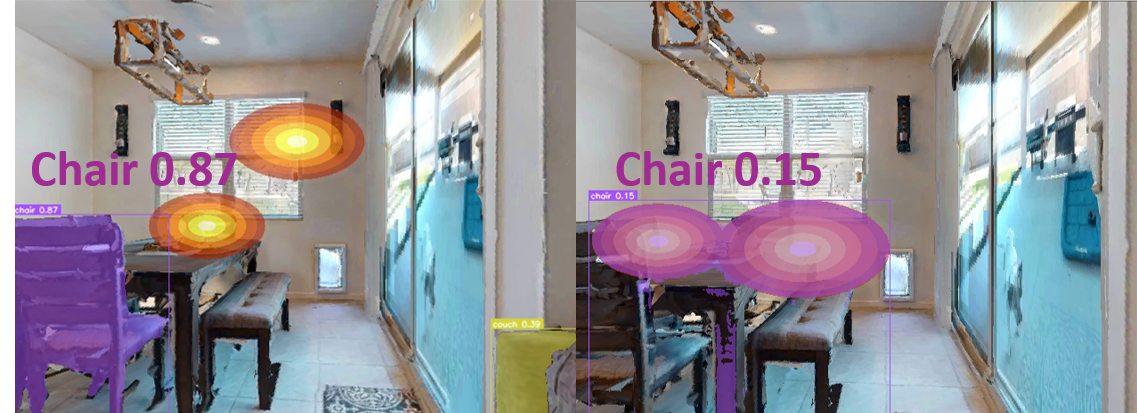
\includegraphics[width=0.382\textwidth]{figures/evaluation/misdetection.png}
%     }
%     \hfill
%     \subfloat[Normal Exploration]{
%         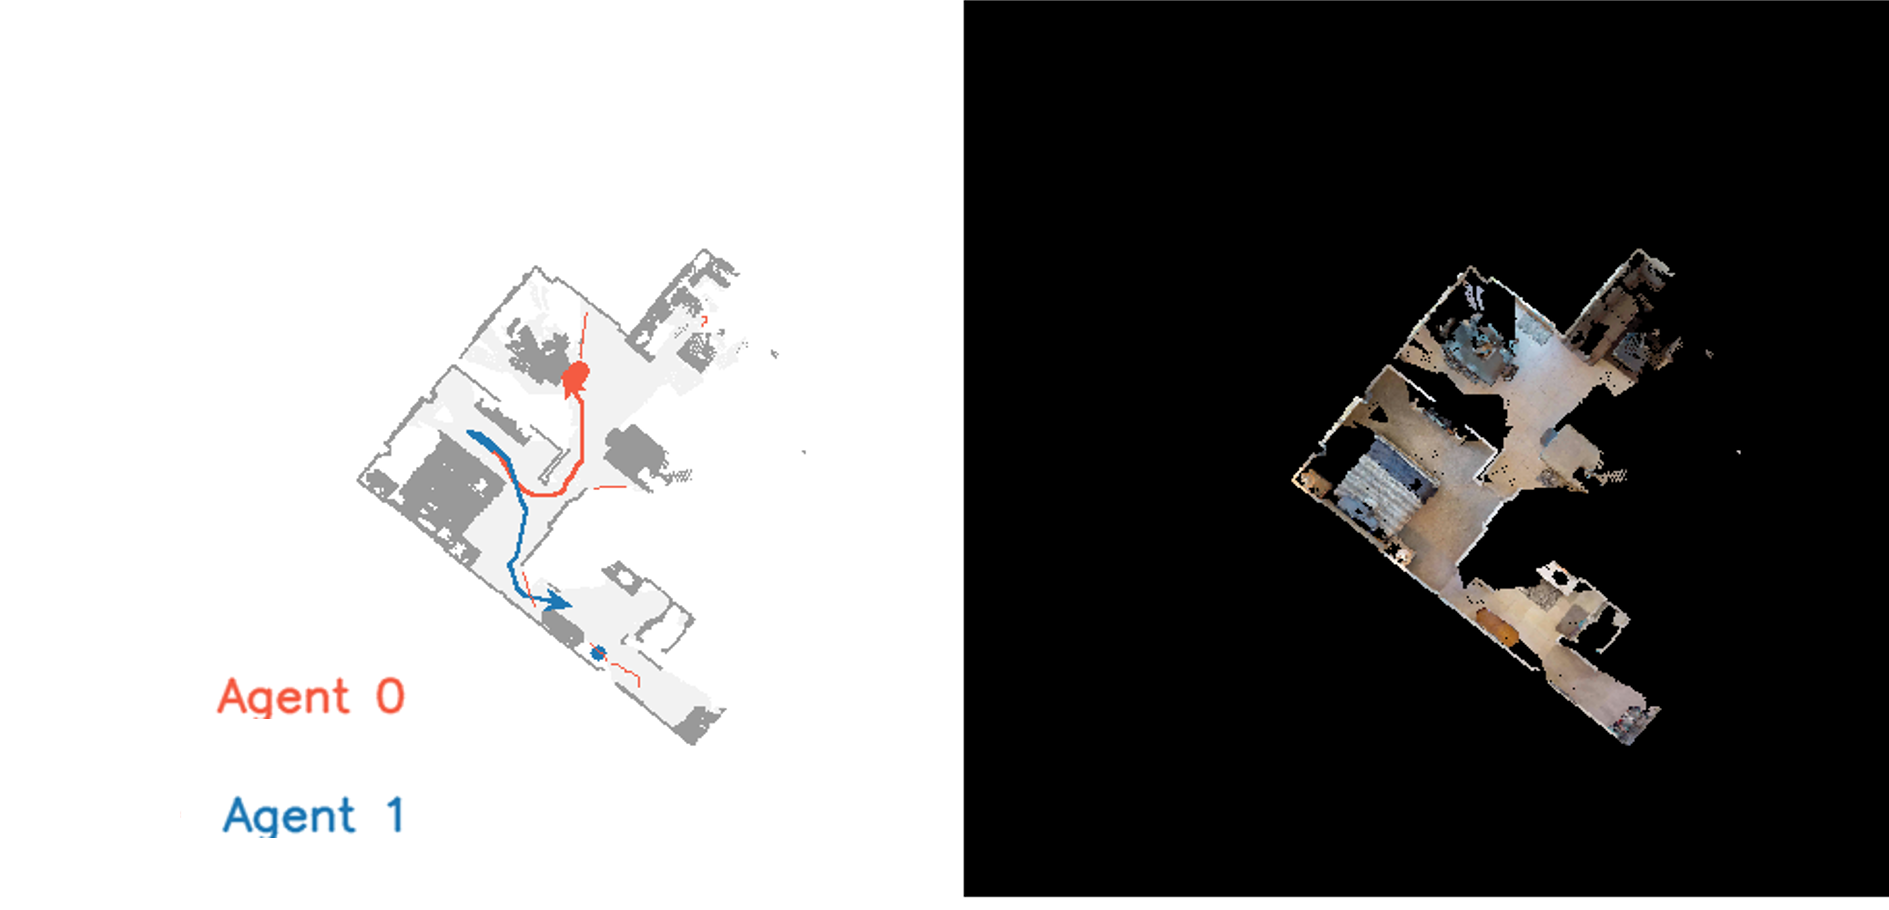
\includegraphics[width=0.29\textwidth]{figures/evaluation/normal_exploration.png}
%     }
%     \hfill
%     \subfloat[Hazard Map]{
%         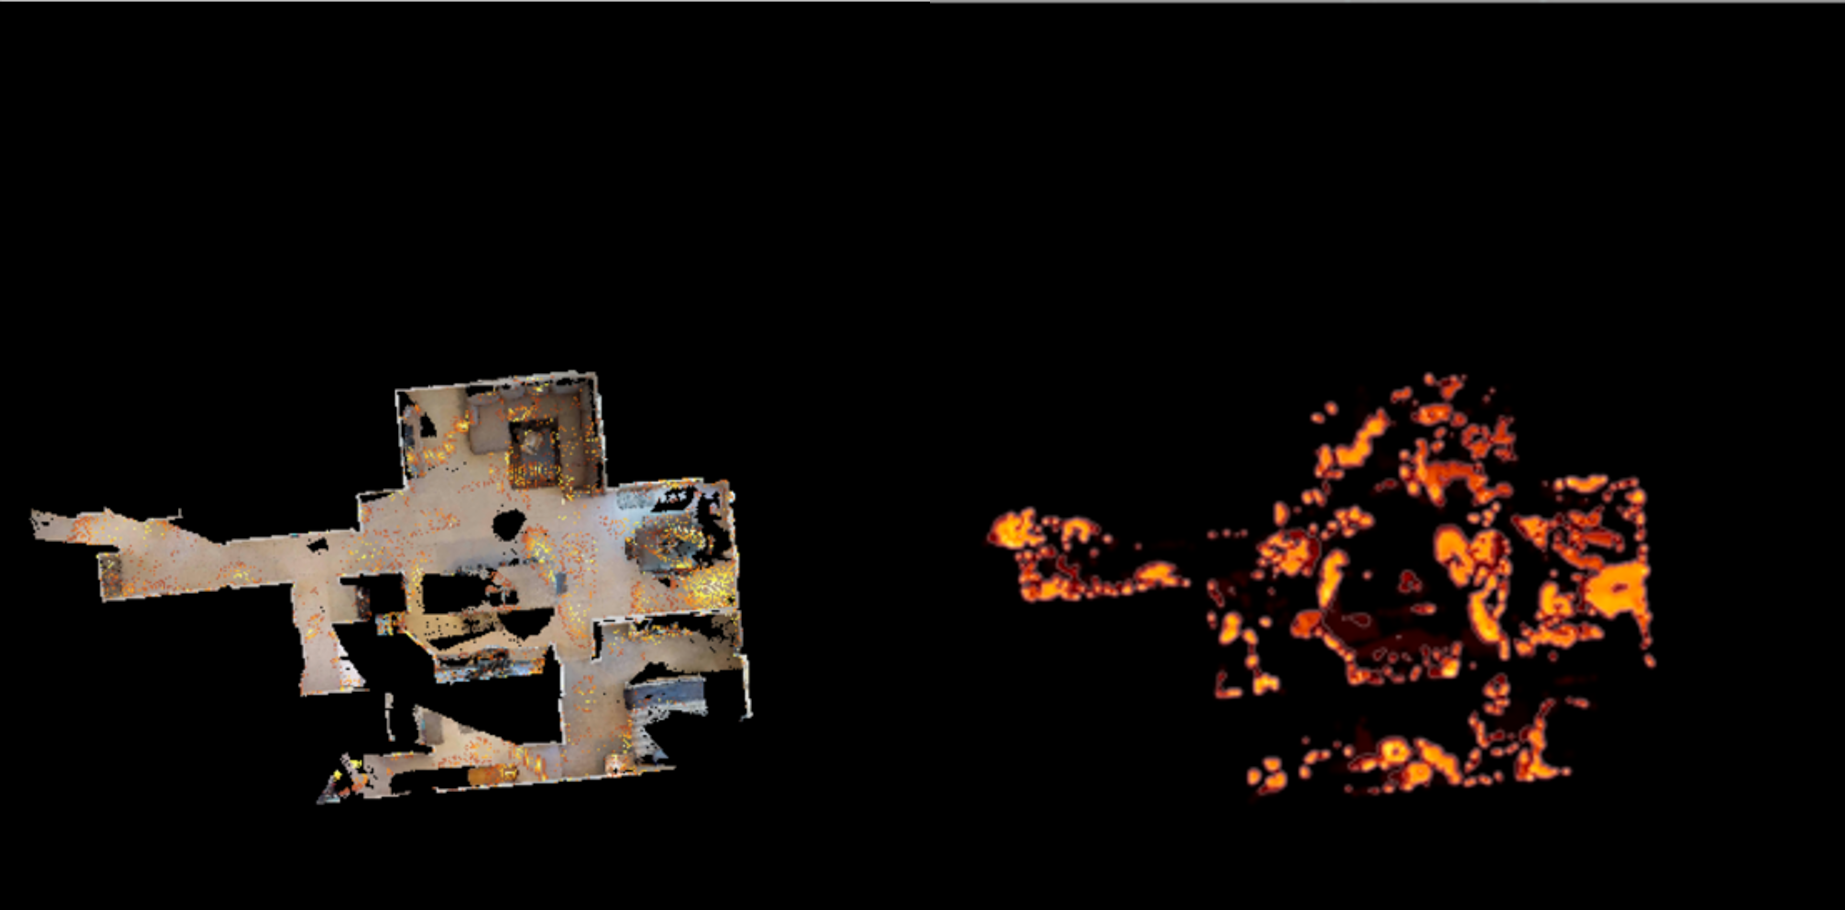
\includegraphics[width=0.283\textwidth]{figures/evaluation/hazard_map.png}
%     }

%     \vspace{0.3cm}

%     % ===== 第二行 =====
%     \subfloat[False detection before and after Fire Scenarios]{
%         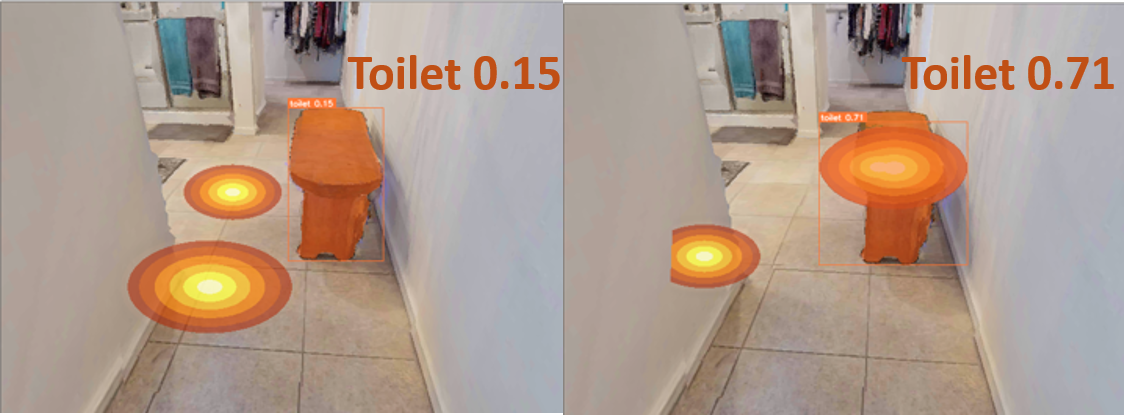
\includegraphics[width=0.382\textwidth]{figures/evaluation/misdetection2.png}
%     }
%     \hfill
%     \subfloat[Fire Exploration]{
%         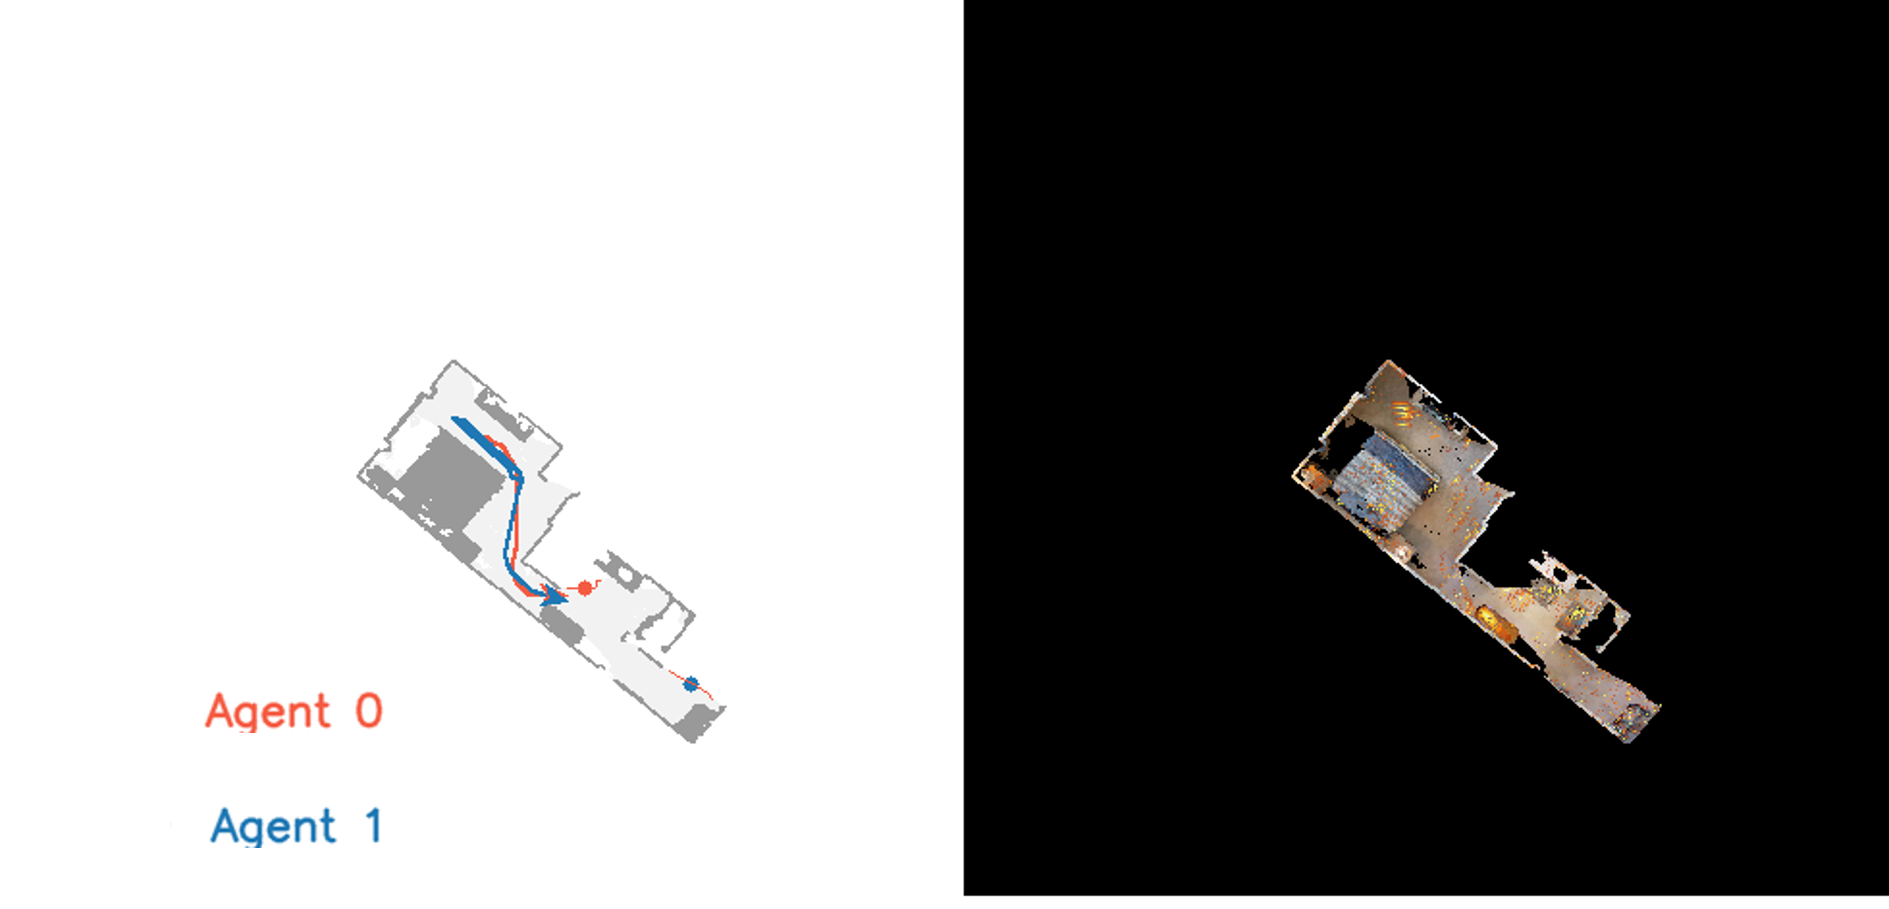
\includegraphics[width=0.29\textwidth]{figures/evaluation/fire_exploration.png}
%     }
%     \hfill
%     \subfloat[False Routing of Entering Fire]{
%         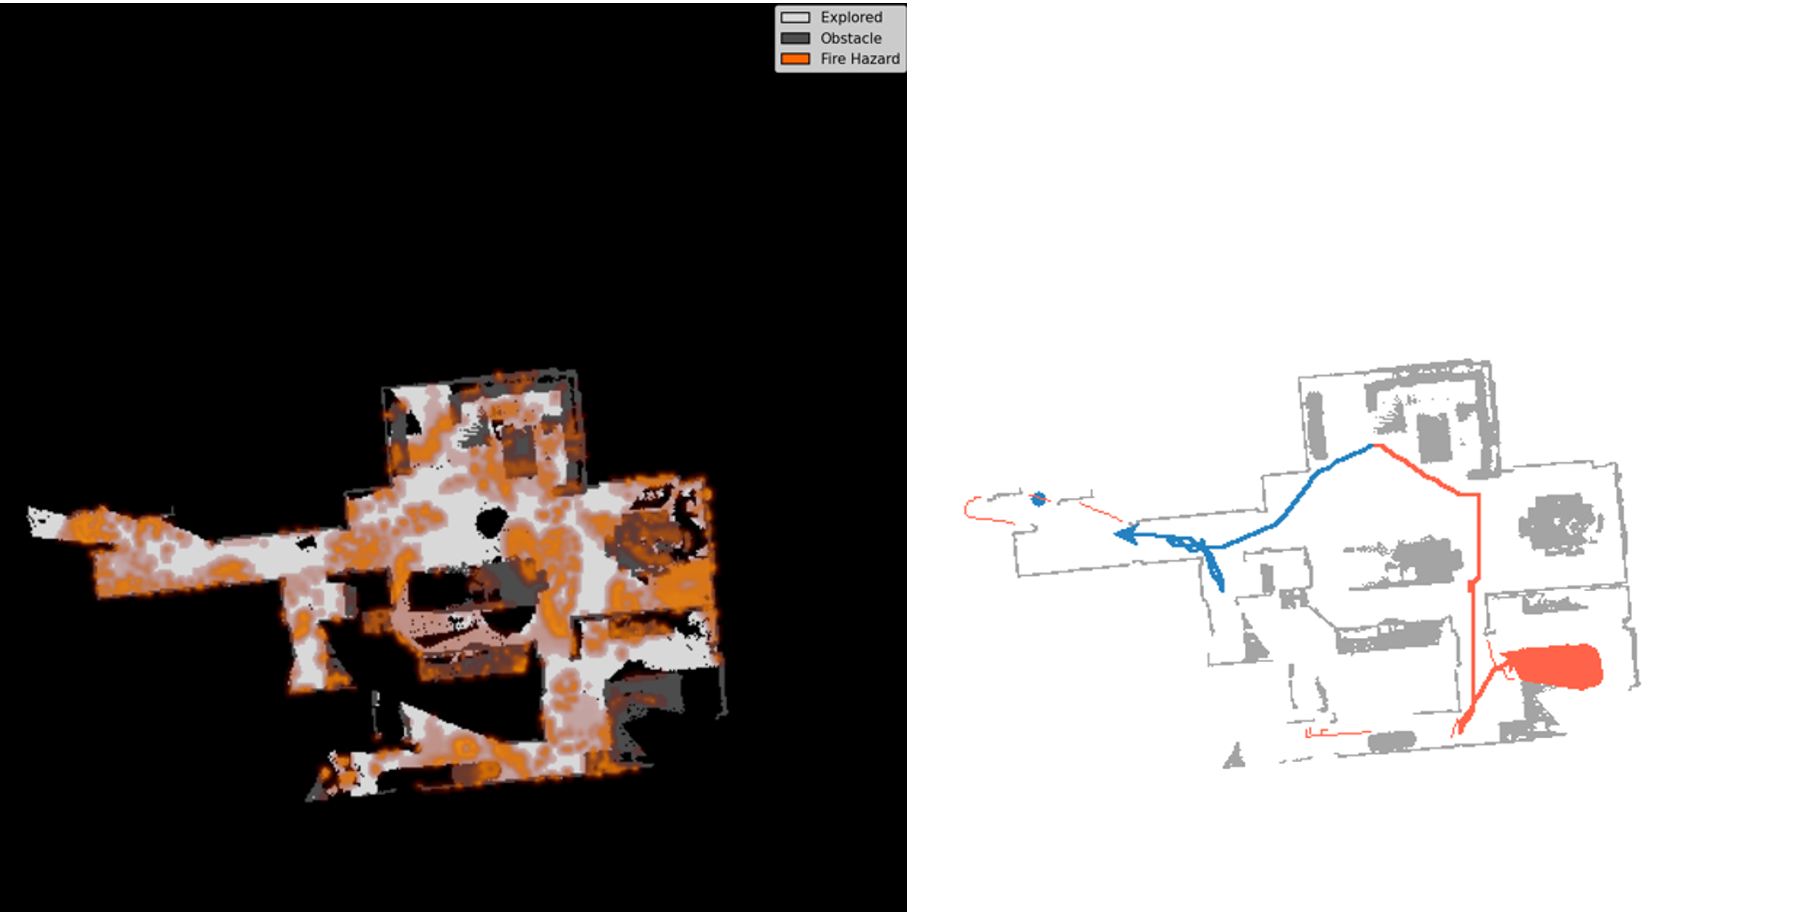
\includegraphics[width=0.283\textwidth]{figures/evaluation/routing_under_fire.png}
%     }

%     \caption{The comparison highlights three failure modes: (a, d) Perception Failure: Smoke causes missed detections (confidence drop in a) and false positives (hallucinations in d); (b, e) Inefficient Exploration: Agents exhibit redundant framing and reduced coverage under fire conditions; (c, f) Unsafe Planning: Without hazard awareness, agents plan paths through high-risk zones (f) despite the presence of thermal hazards shown in the ground-truth map (c).}
%     \label{fig:evaluate_fire}
% \end{figure*}










% \begin{table}[htbp]
%     \centering
%     \caption{Comparative Results Under Normal and Fire Conditions.}
%     \label{tab:comparative_study}
%     \begin{tabular}{l c c c c c c c c}
%         \toprule
%         \multirow{2}{*}{Method} 
%         & \multicolumn{4}{c}{No Fire} 
%         & \multicolumn{4}{c}{Fire} \\
%         \cmidrule(lr){2-5} \cmidrule(lr){6-9}
%         & SR$\uparrow$ & SPL$\uparrow$ & DTG$\downarrow$ & Time$\downarrow$
%         & SR$\uparrow$ & SPL$\uparrow$ & DTG$\downarrow$ & Time$\downarrow$ \\
%         \midrule
%         Greedy 
%         & 0.682 & 0.391 & 1.912 & 1.00
%         & 0.611 & 0.328 & 2.239 & 1.27 \\

%         Cost-Utility 
%         & 0.694 & 0.402 & 1.876 & 1.03
%         & 0.625 & 0.323 & 2.030 & 1.31 \\

%         Random Sample on Map 
%         & 0.701 & 0.410 & 1.842 & 1.05
%         & 0.636 & 0.336 & 2.048 & 1.29 \\

%         Multi-SemExp 
%         & 0.676 & 0.388 & 1.905 & 1.02
%         & 0.612 & 0.327 & 2.234 & 1.34 \\

%         Co-NavGPT 
%         & \textbf{0.732} & \textbf{0.435} & \textbf{1.521} & \textbf{0.94}
%         & \textbf{0.666} & \textbf{0.368} & \textbf{1.684} & \textbf{1.08} \\

%         \bottomrule
%     \end{tabular}
% \end{table}





% In contrast, our approach maintains robust navigation performance by explicitly modeling hazard-aware perception and planning, highlighting the necessity of fire-aware multi-modal reasoning in multi-agent indoor search and rescue scenarios.
